

\tikzset{every picture/.style={line width=0.75pt}} %set default line width to 0.75pt        

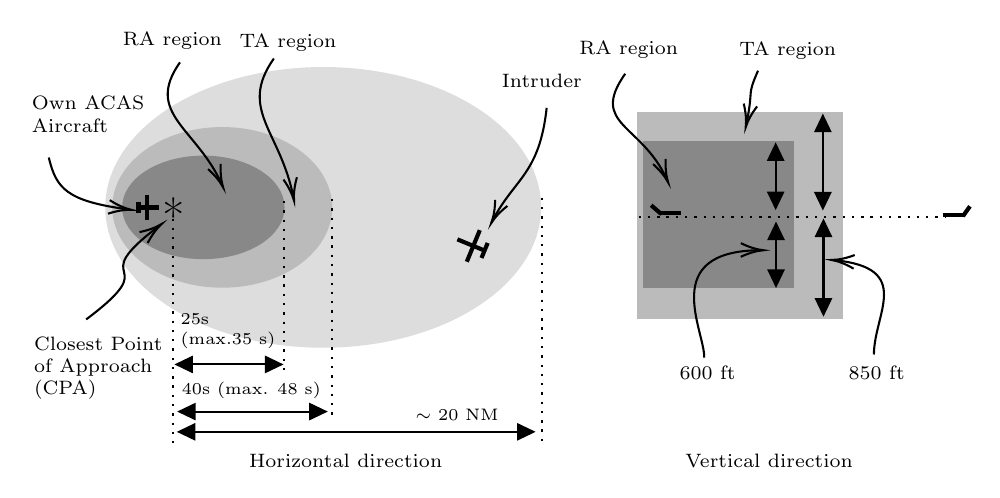
\begin{tikzpicture}[x=0.75pt,y=0.75pt,yscale=-1,xscale=1]
%uncomment if require: \path (0,300); %set diagram left start at 0, and has height of 300

%Shape: Rectangle [id:dp540037046483179] 
\draw  [draw opacity=0][fill={rgb, 255:red, 187; green, 187; blue, 187 }  ,fill opacity=1 ] (306.97,69.51) -- (406.37,69.51) -- (406.37,169.43) -- (306.97,169.43) -- cycle ;
%Shape: Ellipse [id:dp4377400846575308] 
\draw  [draw opacity=0][fill={rgb, 255:red, 221; green, 221; blue, 221 }  ,fill opacity=1 ] (51,115.63) .. controls (51,78.28) and (98.01,48) .. (156,48) .. controls (213.99,48) and (261,78.28) .. (261,115.63) .. controls (261,152.97) and (213.99,183.25) .. (156,183.25) .. controls (98.01,183.25) and (51,152.97) .. (51,115.63) -- cycle ;
%Shape: Ellipse [id:dp13502883869152638] 
\draw  [draw opacity=0][fill={rgb, 255:red, 187; green, 187; blue, 187 }  ,fill opacity=1 ] (54.37,115.63) .. controls (54.37,94.25) and (78.09,76.92) .. (107.35,76.92) .. controls (136.61,76.92) and (160.33,94.25) .. (160.33,115.63) .. controls (160.33,137) and (136.61,154.33) .. (107.35,154.33) .. controls (78.09,154.33) and (54.37,137) .. (54.37,115.63) -- cycle ;
%Shape: Ellipse [id:dp7716523443232073] 
\draw  [draw opacity=0][fill={rgb, 255:red, 136; green, 136; blue, 136 }  ,fill opacity=1 ] (59.13,115.63) .. controls (59.13,101.85) and (76.65,90.68) .. (98.27,90.68) .. controls (119.88,90.68) and (137.4,101.85) .. (137.4,115.63) .. controls (137.4,129.4) and (119.88,140.57) .. (98.27,140.57) .. controls (76.65,140.57) and (59.13,129.4) .. (59.13,115.63) -- cycle ;
%Straight Lines [id:da6234084719762716] 
\draw [line width=0.75]  [dash pattern={on 0.84pt off 2.51pt}]  (83.8,121.03) -- (83.8,231.25) ;
%Straight Lines [id:da986581977231834] 
\draw [line width=0.75]  [dash pattern={on 0.84pt off 2.51pt}]  (137,112.57) -- (137,194.25) ;
%Straight Lines [id:da017080809888795345] 
\draw [line width=0.75]  [dash pattern={on 0.84pt off 2.51pt}]  (160.33,111.63) -- (160.33,216.75) ;
%Straight Lines [id:da9044293647497716] 
\draw [line width=0.75]  [dash pattern={on 0.84pt off 2.51pt}]  (261.5,110.96) -- (261.5,230.25) ;
%Straight Lines [id:da8901469455802469] 
\draw    (87.33,191.29) -- (133.88,191.29) ;
\draw [shift={(136.88,191.29)}, rotate = 180] [fill={rgb, 255:red, 0; green, 0; blue, 0 }  ][line width=0.08]  [draw opacity=0] (8.93,-4.29) -- (0,0) -- (8.93,4.29) -- cycle    ;
\draw [shift={(84.33,191.29)}, rotate = 0] [fill={rgb, 255:red, 0; green, 0; blue, 0 }  ][line width=0.08]  [draw opacity=0] (8.93,-4.29) -- (0,0) -- (8.93,4.29) -- cycle    ;
%Straight Lines [id:da17855104123419885] 
\draw    (88.66,214) -- (155.2,214) ;
\draw [shift={(158.2,214)}, rotate = 180] [fill={rgb, 255:red, 0; green, 0; blue, 0 }  ][line width=0.08]  [draw opacity=0] (8.93,-4.29) -- (0,0) -- (8.93,4.29) -- cycle    ;
\draw [shift={(85.66,214)}, rotate = 0] [fill={rgb, 255:red, 0; green, 0; blue, 0 }  ][line width=0.08]  [draw opacity=0] (8.93,-4.29) -- (0,0) -- (8.93,4.29) -- cycle    ;
%Straight Lines [id:da48115516720549056] 
\draw    (88.48,223.76) -- (255.33,223.76) ;
\draw [shift={(258.33,223.76)}, rotate = 180] [fill={rgb, 255:red, 0; green, 0; blue, 0 }  ][line width=0.08]  [draw opacity=0] (8.93,-4.29) -- (0,0) -- (8.93,4.29) -- cycle    ;
\draw [shift={(85.48,223.76)}, rotate = 0] [fill={rgb, 255:red, 0; green, 0; blue, 0 }  ][line width=0.08]  [draw opacity=0] (8.93,-4.29) -- (0,0) -- (8.93,4.29) -- cycle    ;
%Curve Lines [id:da018523465484951096] 
\draw    (263.67,67.67) .. controls (260.16,99.65) and (248.28,101.59) .. (237.74,121.68) ;
\draw [shift={(236.93,123.27)}, rotate = 296.42] [color={rgb, 255:red, 0; green, 0; blue, 0 }  ][line width=0.75]    (10.93,-3.29) .. controls (6.95,-1.4) and (3.31,-0.3) .. (0,0) .. controls (3.31,0.3) and (6.95,1.4) .. (10.93,3.29)   ;
%Curve Lines [id:da6845841341175849] 
\draw    (132.24,43.9) .. controls (114.79,68.67) and (135.6,78.88) .. (141.68,110.96) ;
\draw [shift={(141.95,112.44)}, rotate = 260.25] [color={rgb, 255:red, 0; green, 0; blue, 0 }  ][line width=0.75]    (10.93,-3.29) .. controls (6.95,-1.4) and (3.31,-0.3) .. (0,0) .. controls (3.31,0.3) and (6.95,1.4) .. (10.93,3.29)   ;
%Curve Lines [id:da9696521875385951] 
\draw    (87,45.75) .. controls (69.64,70.39) and (94.85,77.27) .. (107.07,104.32) ;
\draw [shift={(107.8,106)}, rotate = 247.3] [color={rgb, 255:red, 0; green, 0; blue, 0 }  ][line width=0.75]    (10.93,-3.29) .. controls (6.95,-1.4) and (3.31,-0.3) .. (0,0) .. controls (3.31,0.3) and (6.95,1.4) .. (10.93,3.29)   ;
%Curve Lines [id:da6095777107453137] 
\draw    (41.8,169.6) .. controls (81.4,139.9) and (39.06,153.32) .. (77.02,124.49) ;
\draw [shift={(78.2,123.6)}, rotate = 503.13] [color={rgb, 255:red, 0; green, 0; blue, 0 }  ][line width=0.75]    (10.93,-3.29) .. controls (6.95,-1.4) and (3.31,-0.3) .. (0,0) .. controls (3.31,0.3) and (6.95,1.4) .. (10.93,3.29)   ;
%Curve Lines [id:da5170352565441036] 
\draw    (23.8,91.6) .. controls (27.33,106.5) and (32.39,112.56) .. (61.77,116.56) ;
\draw [shift={(63.6,116.8)}, rotate = 187.35] [color={rgb, 255:red, 0; green, 0; blue, 0 }  ][line width=0.75]    (10.93,-3.29) .. controls (6.95,-1.4) and (3.31,-0.3) .. (0,0) .. controls (3.31,0.3) and (6.95,1.4) .. (10.93,3.29)   ;
%Shape: Rectangle [id:dp533002490009195] 
\draw  [draw opacity=0][fill={rgb, 255:red, 136; green, 136; blue, 136 }  ,fill opacity=1 ] (310.19,83.79) -- (383,83.79) -- (383,154.3) -- (310.19,154.3) -- cycle ;
%Straight Lines [id:da8531155029939488] 
\draw  [dash pattern={on 0.84pt off 2.51pt}]  (308,120.2) -- (455.8,120.2) ;
%Straight Lines [id:da21045740389571743] 
\draw    (396.74,73.46) -- (396.74,114.14) ;
\draw [shift={(396.74,117.14)}, rotate = 270] [fill={rgb, 255:red, 0; green, 0; blue, 0 }  ][line width=0.08]  [draw opacity=0] (8.93,-4.29) -- (0,0) -- (8.93,4.29) -- cycle    ;
\draw [shift={(396.74,70.46)}, rotate = 90] [fill={rgb, 255:red, 0; green, 0; blue, 0 }  ][line width=0.08]  [draw opacity=0] (8.93,-4.29) -- (0,0) -- (8.93,4.29) -- cycle    ;
%Straight Lines [id:da39726982970462643] 
\draw    (397.03,123.97) -- (397.03,165.29) ;
\draw [shift={(397.03,168.29)}, rotate = 270] [fill={rgb, 255:red, 0; green, 0; blue, 0 }  ][line width=0.08]  [draw opacity=0] (8.93,-4.29) -- (0,0) -- (8.93,4.29) -- cycle    ;
\draw [shift={(397.03,120.97)}, rotate = 90] [fill={rgb, 255:red, 0; green, 0; blue, 0 }  ][line width=0.08]  [draw opacity=0] (8.93,-4.29) -- (0,0) -- (8.93,4.29) -- cycle    ;
%Straight Lines [id:da7836831316943322] 
\draw    (374,87.29) -- (374,113.91) ;
\draw [shift={(374,116.91)}, rotate = 270] [fill={rgb, 255:red, 0; green, 0; blue, 0 }  ][line width=0.08]  [draw opacity=0] (8.93,-4.29) -- (0,0) -- (8.93,4.29) -- cycle    ;
\draw [shift={(374,84.29)}, rotate = 90] [fill={rgb, 255:red, 0; green, 0; blue, 0 }  ][line width=0.08]  [draw opacity=0] (8.93,-4.29) -- (0,0) -- (8.93,4.29) -- cycle    ;
%Straight Lines [id:da8366254239434643] 
\draw    (374.17,125.46) -- (374.17,151.46) ;
\draw [shift={(374.17,154.46)}, rotate = 270] [fill={rgb, 255:red, 0; green, 0; blue, 0 }  ][line width=0.08]  [draw opacity=0] (8.93,-4.29) -- (0,0) -- (8.93,4.29) -- cycle    ;
\draw [shift={(374.17,122.46)}, rotate = 90] [fill={rgb, 255:red, 0; green, 0; blue, 0 }  ][line width=0.08]  [draw opacity=0] (8.93,-4.29) -- (0,0) -- (8.93,4.29) -- cycle    ;
%Straight Lines [id:da5952844140181097] 
\draw [line width=1.5]    (317.8,118.4) -- (328.4,118.4) ;
%Straight Lines [id:da8295175050930979] 
\draw [line width=1.5]    (314,114.6) -- (319,118.9) ;

%Straight Lines [id:da04092572822853335] 
\draw [line width=1.5]    (454.6,119.4) -- (465.2,119.4) ;
%Straight Lines [id:da5699307237098779] 
\draw [line width=1.5]    (467.6,115.1) -- (464.2,119.9) ;

%Straight Lines [id:da21934003742303032] 
\draw [line width=1.5]    (66.78,115.67) -- (77.12,115.67) ;
%Straight Lines [id:da0093763820452204] 
\draw [line width=1.5]    (66.99,112.91) -- (66.99,118.5) ;
%Straight Lines [id:da2881776632398887] 
\draw [line width=1.5]    (71.18,109.78) -- (71.18,121.56) ;

%Straight Lines [id:da1381529616415611] 
\draw [line width=1.5]    (234.02,136.54) -- (220.65,131.03) ;
%Straight Lines [id:da8623314816948788] 
\draw [line width=1.5]    (232.27,139.99) -- (235.25,132.76) ;
%Straight Lines [id:da20993063325707295] 
\draw [line width=1.5]    (225.19,141.8) -- (231.46,126.59) ;

%Curve Lines [id:da02921148242050675] 
\draw    (339.57,188) .. controls (339.97,175.33) and (317.18,136.5) .. (366.61,136.26) ;
\draw [shift={(368.13,136.27)}, rotate = 180.62] [color={rgb, 255:red, 0; green, 0; blue, 0 }  ][line width=0.75]    (10.93,-3.29) .. controls (6.95,-1.4) and (3.31,-0.3) .. (0,0) .. controls (3.31,0.3) and (6.95,1.4) .. (10.93,3.29)   ;
%Curve Lines [id:da26674369247427876] 
\draw    (421.33,186.5) .. controls (421.39,166.69) and (440.42,144.95) .. (402.7,141.11) ;
\draw [shift={(400.93,140.95)}, rotate = 364.76] [color={rgb, 255:red, 0; green, 0; blue, 0 }  ][line width=0.75]    (10.93,-3.29) .. controls (6.95,-1.4) and (3.31,-0.3) .. (0,0) .. controls (3.31,0.3) and (6.95,1.4) .. (10.93,3.29)   ;
%Curve Lines [id:da6549261187856048] 
\draw    (301.5,51.25) .. controls (284.14,75.89) and (309.25,75.18) .. (321.47,101.93) ;
\draw [shift={(322.2,103.6)}, rotate = 247.3] [color={rgb, 255:red, 0; green, 0; blue, 0 }  ][line width=0.75]    (10.93,-3.29) .. controls (6.95,-1.4) and (3.31,-0.3) .. (0,0) .. controls (3.31,0.3) and (6.95,1.4) .. (10.93,3.29)   ;
%Curve Lines [id:da058237463472115] 
\draw    (365.5,49.75) .. controls (359.82,62.9) and (363.61,57.09) .. (359.93,75.25) ;
\draw [shift={(359.57,77)}, rotate = 281.93] [color={rgb, 255:red, 0; green, 0; blue, 0 }  ][line width=0.75]    (10.93,-3.29) .. controls (6.95,-1.4) and (3.31,-0.3) .. (0,0) .. controls (3.31,0.3) and (6.95,1.4) .. (10.93,3.29)   ;

% Text Node
\draw (240.6,49.8) node [anchor=north west][inner sep=0.75pt]  [font=\scriptsize] [align=left] {Intruder};
% Text Node
\draw (110.13,185) node [anchor=south] [inner sep=0.75pt]  [font=\fontsize{0.6em}{0.72em}\selectfont] [align=left] {25s\\(max.35 s)};
% Text Node
\draw (121.35,209.34) node [anchor=south] [inner sep=0.75pt]  [font=\fontsize{0.6em}{0.72em}\selectfont] [align=left] {40s (max. 48 s)};
% Text Node
\draw (220.41,219.74) node [anchor=south] [inner sep=0.75pt]  [font=\fontsize{0.6em}{0.72em}\selectfont] [align=left] {$\displaystyle \sim $ 20 NM};
% Text Node
\draw (114.23,30.54) node [anchor=north west][inner sep=0.75pt]  [font=\scriptsize] [align=left] {TA region};
% Text Node
\draw (57.99,29.54) node [anchor=north west][inner sep=0.75pt]  [font=\scriptsize] [align=left] {RA region};
% Text Node
\draw (15.19,176.41) node [anchor=north west][inner sep=0.75pt]  [font=\scriptsize] [align=left] {Closest Point \\of Approach\\(CPA)};
% Text Node
\draw (14.12,60.79) node [anchor=north west][inner sep=0.75pt]  [font=\scriptsize] [align=left] {Own ACAS\\Aircraft};
% Text Node
\draw (326.17,190.48) node [anchor=north west][inner sep=0.75pt]  [font=\scriptsize] [align=left] {600 ft};
% Text Node
\draw (407.66,190.45) node [anchor=north west][inner sep=0.75pt]  [font=\scriptsize] [align=left] {850 ft};
% Text Node
\draw (329,233) node [anchor=north west][inner sep=0.75pt]  [font=\scriptsize] [align=left] {Vertical direction};
% Text Node
\draw (83.8,119.43) node  [font=\LARGE] [align=left] {*};
% Text Node
\draw (277.89,34.04) node [anchor=north west][inner sep=0.75pt]  [font=\scriptsize] [align=left] {RA region};
% Text Node
\draw (354.96,34.54) node [anchor=north west][inner sep=0.75pt]  [font=\scriptsize] [align=left] {TA region};
% Text Node
\draw (118.8,233) node [anchor=north west][inner sep=0.75pt]  [font=\scriptsize] [align=left] {Horizontal direction};


\end{tikzpicture}
